% Options for packages loaded elsewhere
\PassOptionsToPackage{unicode}{hyperref}
\PassOptionsToPackage{hyphens}{url}
%
\documentclass[
  english,
  man]{apa6}
\usepackage{amsmath,amssymb}
\usepackage[]{arev}
\usepackage{ifxetex,ifluatex}
\ifnum 0\ifxetex 1\fi\ifluatex 1\fi=0 % if pdftex
  \usepackage[T1]{fontenc}
  \usepackage[utf8]{inputenc}
  \usepackage{textcomp} % provide euro and other symbols
\else % if luatex or xetex
  \usepackage{unicode-math}
  \defaultfontfeatures{Scale=MatchLowercase}
  \defaultfontfeatures[\rmfamily]{Ligatures=TeX,Scale=1}
\fi
% Use upquote if available, for straight quotes in verbatim environments
\IfFileExists{upquote.sty}{\usepackage{upquote}}{}
\IfFileExists{microtype.sty}{% use microtype if available
  \usepackage[]{microtype}
  \UseMicrotypeSet[protrusion]{basicmath} % disable protrusion for tt fonts
}{}
\makeatletter
\@ifundefined{KOMAClassName}{% if non-KOMA class
  \IfFileExists{parskip.sty}{%
    \usepackage{parskip}
  }{% else
    \setlength{\parindent}{0pt}
    \setlength{\parskip}{6pt plus 2pt minus 1pt}}
}{% if KOMA class
  \KOMAoptions{parskip=half}}
\makeatother
\usepackage{xcolor}
\IfFileExists{xurl.sty}{\usepackage{xurl}}{} % add URL line breaks if available
\IfFileExists{bookmark.sty}{\usepackage{bookmark}}{\usepackage{hyperref}}
\hypersetup{
  pdftitle={Light Exposure Behavior Assessment (LEBA): Develop of a novel instrument to capture light exposure-related behaviours},
  pdfauthor={Mushfiqul Anwar Siraji1, Rafael Robert Lazar2, \& Manuel Spitschan3},
  pdflang={en-EN},
  pdfkeywords={keywords},
  hidelinks,
  pdfcreator={LaTeX via pandoc}}
\urlstyle{same} % disable monospaced font for URLs
\usepackage{graphicx}
\makeatletter
\def\maxwidth{\ifdim\Gin@nat@width>\linewidth\linewidth\else\Gin@nat@width\fi}
\def\maxheight{\ifdim\Gin@nat@height>\textheight\textheight\else\Gin@nat@height\fi}
\makeatother
% Scale images if necessary, so that they will not overflow the page
% margins by default, and it is still possible to overwrite the defaults
% using explicit options in \includegraphics[width, height, ...]{}
\setkeys{Gin}{width=\maxwidth,height=\maxheight,keepaspectratio}
% Set default figure placement to htbp
\makeatletter
\def\fps@figure{htbp}
\makeatother
\setlength{\emergencystretch}{3em} % prevent overfull lines
\providecommand{\tightlist}{%
  \setlength{\itemsep}{0pt}\setlength{\parskip}{0pt}}
\setcounter{secnumdepth}{-\maxdimen} % remove section numbering
% Make \paragraph and \subparagraph free-standing
\ifx\paragraph\undefined\else
  \let\oldparagraph\paragraph
  \renewcommand{\paragraph}[1]{\oldparagraph{#1}\mbox{}}
\fi
\ifx\subparagraph\undefined\else
  \let\oldsubparagraph\subparagraph
  \renewcommand{\subparagraph}[1]{\oldsubparagraph{#1}\mbox{}}
\fi
% Manuscript styling
\usepackage{upgreek}
\captionsetup{font=singlespacing,justification=justified}

% Table formatting
\usepackage{longtable}
\usepackage{lscape}
% \usepackage[counterclockwise]{rotating}   % Landscape page setup for large tables
\usepackage{multirow}		% Table styling
\usepackage{tabularx}		% Control Column width
\usepackage[flushleft]{threeparttable}	% Allows for three part tables with a specified notes section
\usepackage{threeparttablex}            % Lets threeparttable work with longtable

% Create new environments so endfloat can handle them
% \newenvironment{ltable}
%   {\begin{landscape}\begin{center}\begin{threeparttable}}
%   {\end{threeparttable}\end{center}\end{landscape}}
\newenvironment{lltable}{\begin{landscape}\begin{center}\begin{ThreePartTable}}{\end{ThreePartTable}\end{center}\end{landscape}}

% Enables adjusting longtable caption width to table width
% Solution found at http://golatex.de/longtable-mit-caption-so-breit-wie-die-tabelle-t15767.html
\makeatletter
\newcommand\LastLTentrywidth{1em}
\newlength\longtablewidth
\setlength{\longtablewidth}{1in}
\newcommand{\getlongtablewidth}{\begingroup \ifcsname LT@\roman{LT@tables}\endcsname \global\longtablewidth=0pt \renewcommand{\LT@entry}[2]{\global\advance\longtablewidth by ##2\relax\gdef\LastLTentrywidth{##2}}\@nameuse{LT@\roman{LT@tables}} \fi \endgroup}

% \setlength{\parindent}{0.5in}
% \setlength{\parskip}{0pt plus 0pt minus 0pt}

% Overwrite redefinition of paragraph and subparagraph by the default LaTeX template
% See https://github.com/crsh/papaja/issues/292
\makeatletter
\renewcommand{\paragraph}{\@startsection{paragraph}{4}{\parindent}%
  {0\baselineskip \@plus 0.2ex \@minus 0.2ex}%
  {-1em}%
  {\normalfont\normalsize\bfseries\itshape\typesectitle}}

\renewcommand{\subparagraph}[1]{\@startsection{subparagraph}{5}{1em}%
  {0\baselineskip \@plus 0.2ex \@minus 0.2ex}%
  {-\z@\relax}%
  {\normalfont\normalsize\itshape\hspace{\parindent}{#1}\textit{\addperi}}{\relax}}
\makeatother

% \usepackage{etoolbox}
\makeatletter
\patchcmd{\HyOrg@maketitle}
  {\section{\normalfont\normalsize\abstractname}}
  {\section*{\normalfont\normalsize\abstractname}}
  {}{\typeout{Failed to patch abstract.}}
\patchcmd{\HyOrg@maketitle}
  {\section{\protect\normalfont{\@title}}}
  {\section*{\protect\normalfont{\@title}}}
  {}{\typeout{Failed to patch title.}}
\makeatother
\shorttitle{LEBA}
\keywords{keywords\newline\indent Word count: X}
\DeclareDelayedFloatFlavor{ThreePartTable}{table}
\DeclareDelayedFloatFlavor{lltable}{table}
\DeclareDelayedFloatFlavor*{longtable}{table}
\makeatletter
\renewcommand{\efloat@iwrite}[1]{\immediate\expandafter\protected@write\csname efloat@post#1\endcsname{}}
\makeatother
\usepackage{lineno}

\linenumbers
\usepackage{csquotes}
\ifxetex
  % Load polyglossia as late as possible: uses bidi with RTL langages (e.g. Hebrew, Arabic)
  \usepackage{polyglossia}
  \setmainlanguage[]{english}
\else
  \usepackage[main=english]{babel}
% get rid of language-specific shorthands (see #6817):
\let\LanguageShortHands\languageshorthands
\def\languageshorthands#1{}
\fi
\ifluatex
  \usepackage{selnolig}  % disable illegal ligatures
\fi
\newlength{\cslhangindent}
\setlength{\cslhangindent}{1.5em}
\newlength{\csllabelwidth}
\setlength{\csllabelwidth}{3em}
\newenvironment{CSLReferences}[2] % #1 hanging-ident, #2 entry spacing
 {% don't indent paragraphs
  \setlength{\parindent}{0pt}
  % turn on hanging indent if param 1 is 1
  \ifodd #1 \everypar{\setlength{\hangindent}{\cslhangindent}}\ignorespaces\fi
  % set entry spacing
  \ifnum #2 > 0
  \setlength{\parskip}{#2\baselineskip}
  \fi
 }%
 {}
\usepackage{calc}
\newcommand{\CSLBlock}[1]{#1\hfill\break}
\newcommand{\CSLLeftMargin}[1]{\parbox[t]{\csllabelwidth}{#1}}
\newcommand{\CSLRightInline}[1]{\parbox[t]{\linewidth - \csllabelwidth}{#1}\break}
\newcommand{\CSLIndent}[1]{\hspace{\cslhangindent}#1}

\title{\emph{Light Exposure Behavior Assessment (LEBA)}: Develop of a novel instrument to capture light exposure-related behaviours}
\author{Mushfiqul Anwar Siraji\textsuperscript{1}, Rafael Robert Lazar\textsuperscript{2}, \& Manuel Spitschan\textsuperscript{3}}
\date{}


\authornote{

Add complete departmental affiliations for each author here. Each new line herein must be indented, like this line.

Enter author note here.

The authors made the following contributions. Mushfiqul Anwar Siraji: Data Analysis, Writing - Original Draft Preparation, Data Visualization; Rafael Robert Lazar: Data Analysis, Writing - Original Draft Preparation, Data Visualization; Manuel Spitschan: Data Analysis, Writing - Original Draft Preparation, Data Visualization.

Correspondence concerning this article should be addressed to Manuel Spitschan, . E-mail:

}

\affiliation{\vspace{0.5cm}\textsuperscript{1} Department of Psychology, Jeffrey Cheah School of Medicine and Health Sciences, Monash University, Malaysia\\\textsuperscript{2} University of Basel}

\abstract{
One or two sentences providing a \textbf{basic introduction} to the field, comprehensible to a scientist in any discipline.

Two to three sentences of \textbf{more detailed background}, comprehensible to scientists in related disciplines.

One sentence clearly stating the \textbf{general problem} being addressed by this particular study.

One sentence summarizing the main result (with the words ``\textbf{here we show}'' or their equivalent).

Two or three sentences explaining what the \textbf{main result} reveals in direct comparison to what was thought to be the case previously, or how the main result adds to previous knowledge.

One or two sentences to put the results into a more \textbf{general context}.

Two or three sentences to provide a \textbf{broader perspective}, readily comprehensible to a scientist in any discipline.
}



\begin{document}
\maketitle

\hypertarget{introduction}{%
\section{Introduction}\label{introduction}}

\hypertarget{methods}{%
\section{Methods}\label{methods}}

\hypertarget{participants}{%
\subsection{Participants}\label{participants}}

\begin{enumerate}
\def\labelenumi{\arabic{enumi}.}
\tightlist
\item
  Describe EFA and CFA sample separately.
\item
  Sampling technique: Convince sampling (non-probability sample)
\item
  Method: cross-sectional survey
\item
  How many missing data?
\item
  How incomplete data were addressed.
\item
  Why such sample was chosen?
\end{enumerate}

EFA: For exploring initial factor structure, a sample of 250-300 is recommended (Comrey \& Lee, 1992; Schönbrodt \& Perugini, 2013)

CFA: For estimating the sample size for the confirmatory factor analysis we followed the N:q rule (Bentler \& Chou, 1987; Jackson, 2003; Kline, 2015; Worthington \& Whittaker, 2006) where 10 participants per parameters is required to earn trustworthiness of the result. Our sample size exceeds the requirement.

\hypertarget{procedure}{%
\subsection{Procedure}\label{procedure}}

\hypertarget{development-of-the-scale}{%
\subsubsection{Development of the Scale}\label{development-of-the-scale}}

\begin{enumerate}
\def\labelenumi{\arabic{enumi}.}
\tightlist
\item
  How the items were generated
\item
  How the literature was reviewed to identify construct adequacy of the items.
\item
  Discuss the expert panel review process to assess content validity
\end{enumerate}

\begin{figure}

{\centering 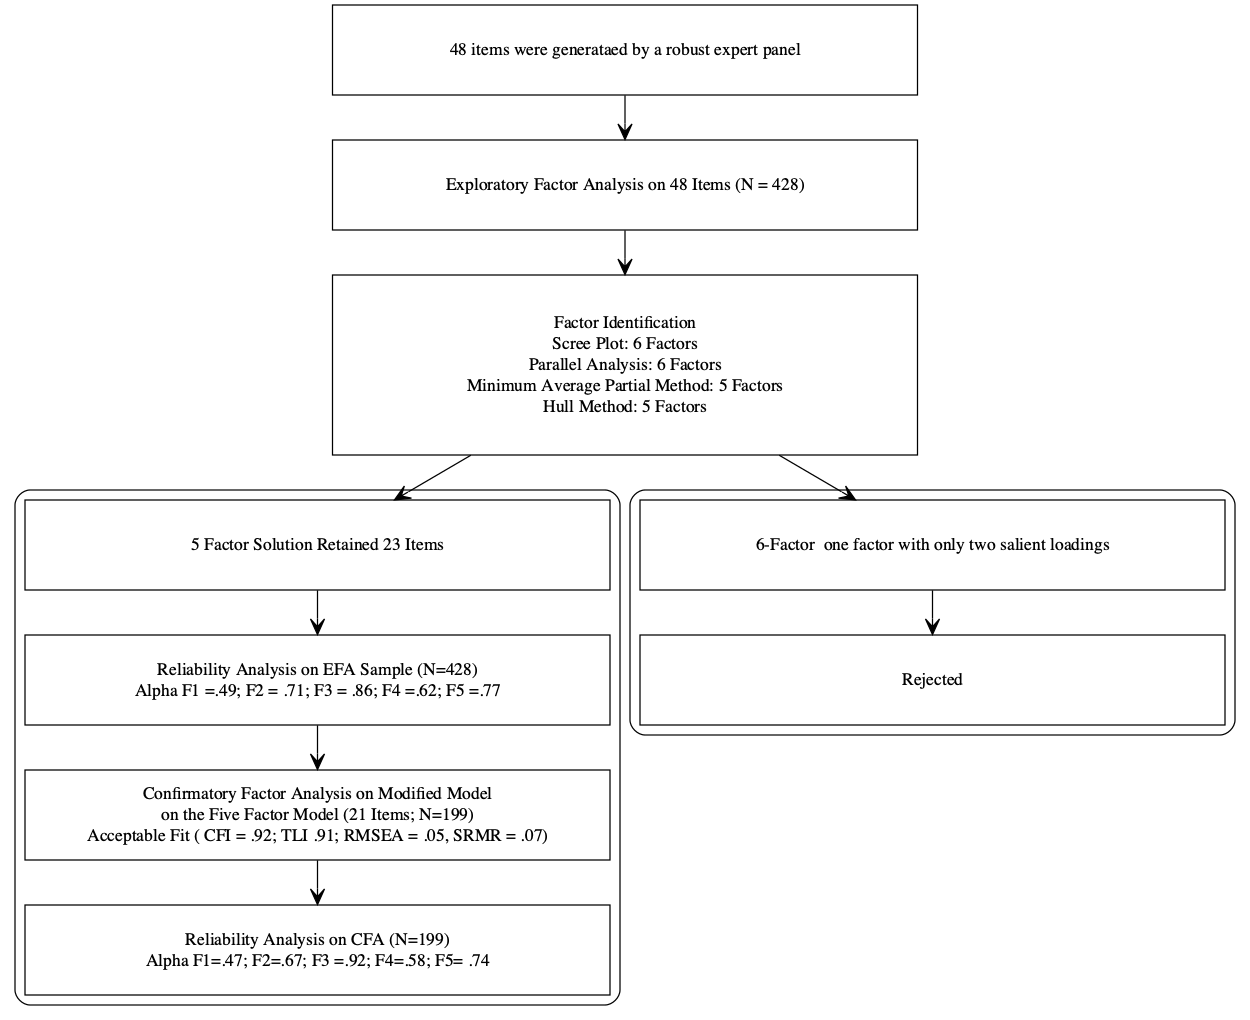
\includegraphics[width=1\linewidth,height=1\textheight]{Flowchart1} 

}

\caption{Development and psychometric properties of LEBA }\label{fig:unnamed-chunk-1}
\end{figure}

\hypertarget{procedure-1}{%
\subsection{Procedure}\label{procedure-1}}

Our study had four objectives. First, to develop an instrument to assess an individual's light exposure behavior. Second, to conduct an exploratory factor analysis(EFA) to understand the latent structure. The third one is to gather structural validity evidence for the latent structure obtained in EFA. Lastly, we gathered item information using Item response theory (IRT)(Baker, 2017)

\hypertarget{data-collection}{%
\subsubsection{Data Collection}\label{data-collection}}

Timeline of data collection,
ethical approval
mode of data collection
how consent was recorded.

\hypertarget{analytic-strategies}{%
\subsection{Analytic Strategies}\label{analytic-strategies}}

We used R (version 4.1.0), including several R packages, for our analyses. Necessary assumptions of EFA, including sample adequacy, normality assumptions, quality of correlation matrix, were assessed. Our data violated both the univariate and multivariate normality assumptions. Due to these violations and the ordinal nature of our response data, we used a polychoric correlation matrix (C. Desjardins \& Bulut, 2018) for the EFA. We employed principal axis (pa) a factor extraction method with varimax rotation. PA is robust to the normality assumption violations (Watkins, 2020). The obtained latent structure was confirmed by the minimum residuals extraction method as well. We used a combination factor identification method including scree plot(Cattell, 1966), Horn's parallel analysis (Horn, 1965), minimum average partials method(Velicer, 1976), and hull method (Lorenzo-Seva, Timmerman, \& Kiers, 2011) to identify factor numbers. Additionally, to determine the simple structure, we followed the following guidelines recommended by psychometricians (i) no factors with fewer than three items (ii) no factors with a factor loading \textless0.3 (iii) no items with cross-loading greater than .3 across factors {[}Bandalos and Finney (2018);

\hypertarget{results}{%
\section{Results}\label{results}}

Sampling adequacy was checked using Kaiser-Meyer-Olkin (KMO) measures of sampling adequacy(Kaiser, 1974) . The overall KMO vale for 48 items was 0.63 which was above the cutoff value (.50) indicating a mediocre sample (Hutcheson, 1999).

\begin{center}
\begin{ThreePartTable}

\begin{TableNotes}[para]
\normalsize{\textit{Note.} *p<.001}
\end{TableNotes}

\begin{longtable}{ccccccc}\noalign{\getlongtablewidth\global\LTcapwidth=\longtablewidth}
\caption{\label{tab:tabDes}Descriptive Statistics}\\
\toprule
 & \multicolumn{1}{c}{Mean} & \multicolumn{1}{c}{SD} & \multicolumn{1}{c}{Skew} & \multicolumn{1}{c}{Kurtosis} & \multicolumn{1}{c}{Shapiro-Wilk Statistics} & \multicolumn{1}{c}{Item-Total Correlation}\\
\midrule
\endfirsthead
\caption*{\normalfont{Table \ref{tab:tabDes} continued}}\\
\toprule
 & \multicolumn{1}{c}{Mean} & \multicolumn{1}{c}{SD} & \multicolumn{1}{c}{Skew} & \multicolumn{1}{c}{Kurtosis} & \multicolumn{1}{c}{Shapiro-Wilk Statistics} & \multicolumn{1}{c}{Item-Total Correlation}\\
\midrule
\endhead
Item1 & 1.12 & 0.49 & 5.02 & 27.80 & 0.25* & .16\\
Item2 & 2.16 & 1.19 & 0.71 & -0.54 & 0.84* & .14\\
Item3 & 4.14 & 0.99 & -1.23 & 1.14 & 0.79* & .19\\
Item4 & 2.87 & 1.59 & 0.08 & -1.60 & 0.83* & .19\\
Item5 & 1.76 & 1.23 & 1.35 & 0.44 & 0.66* & .38\\
Item6 & 2.73 & 1.46 & 0.20 & -1.36 & 0.87* & .33\\
Item7 & 3.86 & 1.67 & -0.99 & -0.85 & 0.65* & .23\\
Item8 & 3.76 & 1.14 & -0.68 & -0.45 & 0.86* & .00\\
Item9 & 3.42 & 1.83 & -0.45 & -1.69 & 0.69* & .33\\
Item10 & 2.74 & 1.04 & 0.09 & -0.74 & 0.91* & .28\\
Item11 & 2.60 & 1.25 & 0.29 & -0.86 & 0.89* & .35\\
Item12 & 2.11 & 1.17 & 0.77 & -0.39 & 0.83* & .32\\
Item13 & 2.94 & 1.03 & -0.12 & -0.40 & 0.91* & .10\\
Item14 & 3.62 & 1.64 & -0.68 & -1.25 & 0.74* & .32\\
Item15 & 1.64 & 1.18 & 1.79 & 2.02 & 0.60* & .15\\
Item16 & 3.51 & 1.30 & -0.70 & -0.59 & 0.85* & .39\\
Item17 & 1.96 & 0.98 & 1.02 & 0.69 & 0.82* & .05\\
Item18 & 2.44 & 1.31 & 0.38 & -1.14 & 0.86* & .11\\
Item19 & 3.80 & 1.29 & -0.87 & -0.42 & 0.82* & .17\\
Item20 & 4.01 & 1.40 & -1.22 & 0.07 & 0.70* & .13\\
Item21 & 1.33 & 0.91 & 3.03 & 8.43 & 0.41* & .01\\
Item22 & 2.59 & 1.41 & 0.27 & -1.27 & 0.86* & .19\\
Item23 & 1.31 & 0.81 & 2.75 & 6.92 & 0.43* & .21\\
Item24 & 1.47 & 1.18 & 2.38 & 4.00 & 0.43* & .28\\
Item25 & 2.56 & 1.27 & 0.33 & -1.00 & 0.89* & .11\\
Item26 & 1.54 & 1.25 & 2.13 & 2.86 & 0.46* & .36\\
Item27 & 4.30 & 1.08 & -1.79 & 2.53 & 0.67* & .22\\
Item28 & 2.27 & 1.39 & 0.74 & -0.81 & 0.81* & .25\\
Item29 & 3.26 & 1.09 & -0.26 & -0.45 & 0.91* & .14\\
Item30 & 2.22 & 1.48 & 0.71 & -1.02 & 0.76* & .30\\
Item31 & 1.05 & 0.36 & 7.23 & 52.98 & 0.13* & .18\\
Item32 & 1.54 & 1.21 & 2.07 & 2.75 & 0.49* & .31\\
Item33 & 1.04 & 0.33 & 8.99 & 85.28 & 0.10* & .16\\
Item34 & 3.36 & 1.38 & -0.48 & -1.03 & 0.87* & .16\\
Item35 & 2.26 & 1.25 & 0.70 & -0.60 & 0.85* & .19\\
Item36 & 2.36 & 1.22 & 0.59 & -0.62 & 0.87* & .25\\
Item37 & 1.14 & 0.59 & 4.79 & 24.05 & 0.25* & .16\\
Item38 & 2.25 & 1.27 & 0.69 & -0.64 & 0.84* & .18\\
Item39 & 3.93 & 1.48 & -1.06 & -0.44 & 0.71* & .18\\
Item40 & 3.57 & 1.07 & -0.65 & -0.17 & 0.88* & .21\\
Item41 & 3.55 & 1.65 & -0.60 & -1.34 & 0.76* & .43\\
Item42 & 3.00 & 1.62 & -0.08 & -1.61 & 0.83* & .44\\
Item43 & 1.56 & 1.23 & 2.00 & 2.45 & 0.50* & .32\\
Item44 & 2.97 & 1.20 & -0.06 & -0.94 & 0.91* & -.10\\
Item45 & 2.79 & 1.55 & 0.19 & -1.48 & 0.85* & .20\\
Item46 & 2.14 & 1.31 & 0.77 & -0.78 & 0.80* & .26\\
Item47 & 2.18 & 0.90 & 0.60 & 0.12 & 0.86* & .26\\
Item48 & 1.48 & 1.11 & 2.18 & 3.35 & 0.48* & .24\\
\bottomrule
\addlinespace
\insertTableNotes
\end{longtable}

\end{ThreePartTable}
\end{center}

\begin{figure}

{\centering 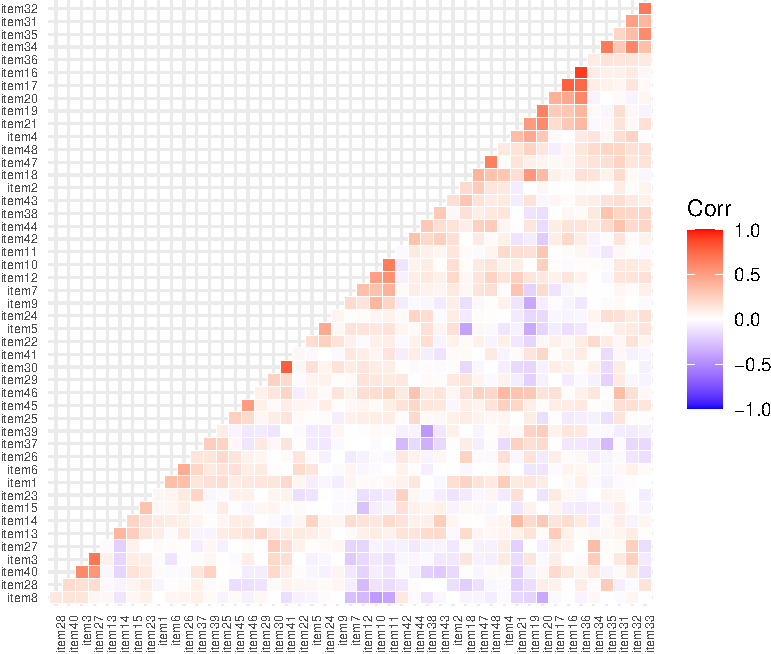
\includegraphics[width=0.5\linewidth]{manuscript_files/figure-latex/figCor-1} 

}

\caption{Correlation plot of the items}\label{fig:figCor}
\end{figure}

Table\ref{tab:tabDes} summarizes the univariate descriptive statistics for the 48 items. some of the items were skewed with high Kurtosis values. Our data violated both univariate normality (Shapiro-Wilk statistics; (Shapiro \& Wilk, 1965)) and multivariate normality assumptions (Marida's test;(Mardia, 1970)). Multivariate skew was = 583.80 (p \textless0.001) and multivariate kurtosis was = 2,749.15 (p \textless0.001). Due to these violations and ordinal nature of the response data polychoric correlations over Pearson's correlations was chosen (C. Desjardins \& Bulut, 2018). Bartlett's test of sphericity (Bartlett, 1954), \(\chi^2\) (1128) = 5042.86, p \textless{} .001{]} indicated the correlations between items are adequate for the EFA. However only 4.96\% of the inter-item correlation coefficients were greater than .30. The inter item correlation ranged between .44 to .91. And the corrected item-total correlations ranged between .10 to .44.

Scree plot ( Figure \ref{fig:facid}) suggested a six-factor solution. Horn's parallel analysis (Horn, 1965) with 500 iterations also indicated a six-factor solution. However, the MAP method (Velicer, 1976) and Hull method (Lorenzo-Seva, Timmerman, \& Kiers, 2011) suggested a five-factor solution. As a result, we tested both five-factor and six-factor solutions.

\begin{figure}

{\centering 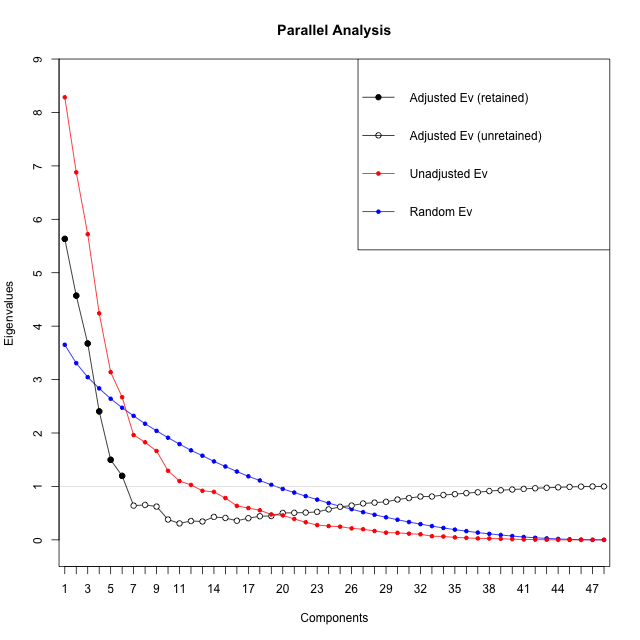
\includegraphics[width=0.5\linewidth,height=0.5\textheight]{parallel} 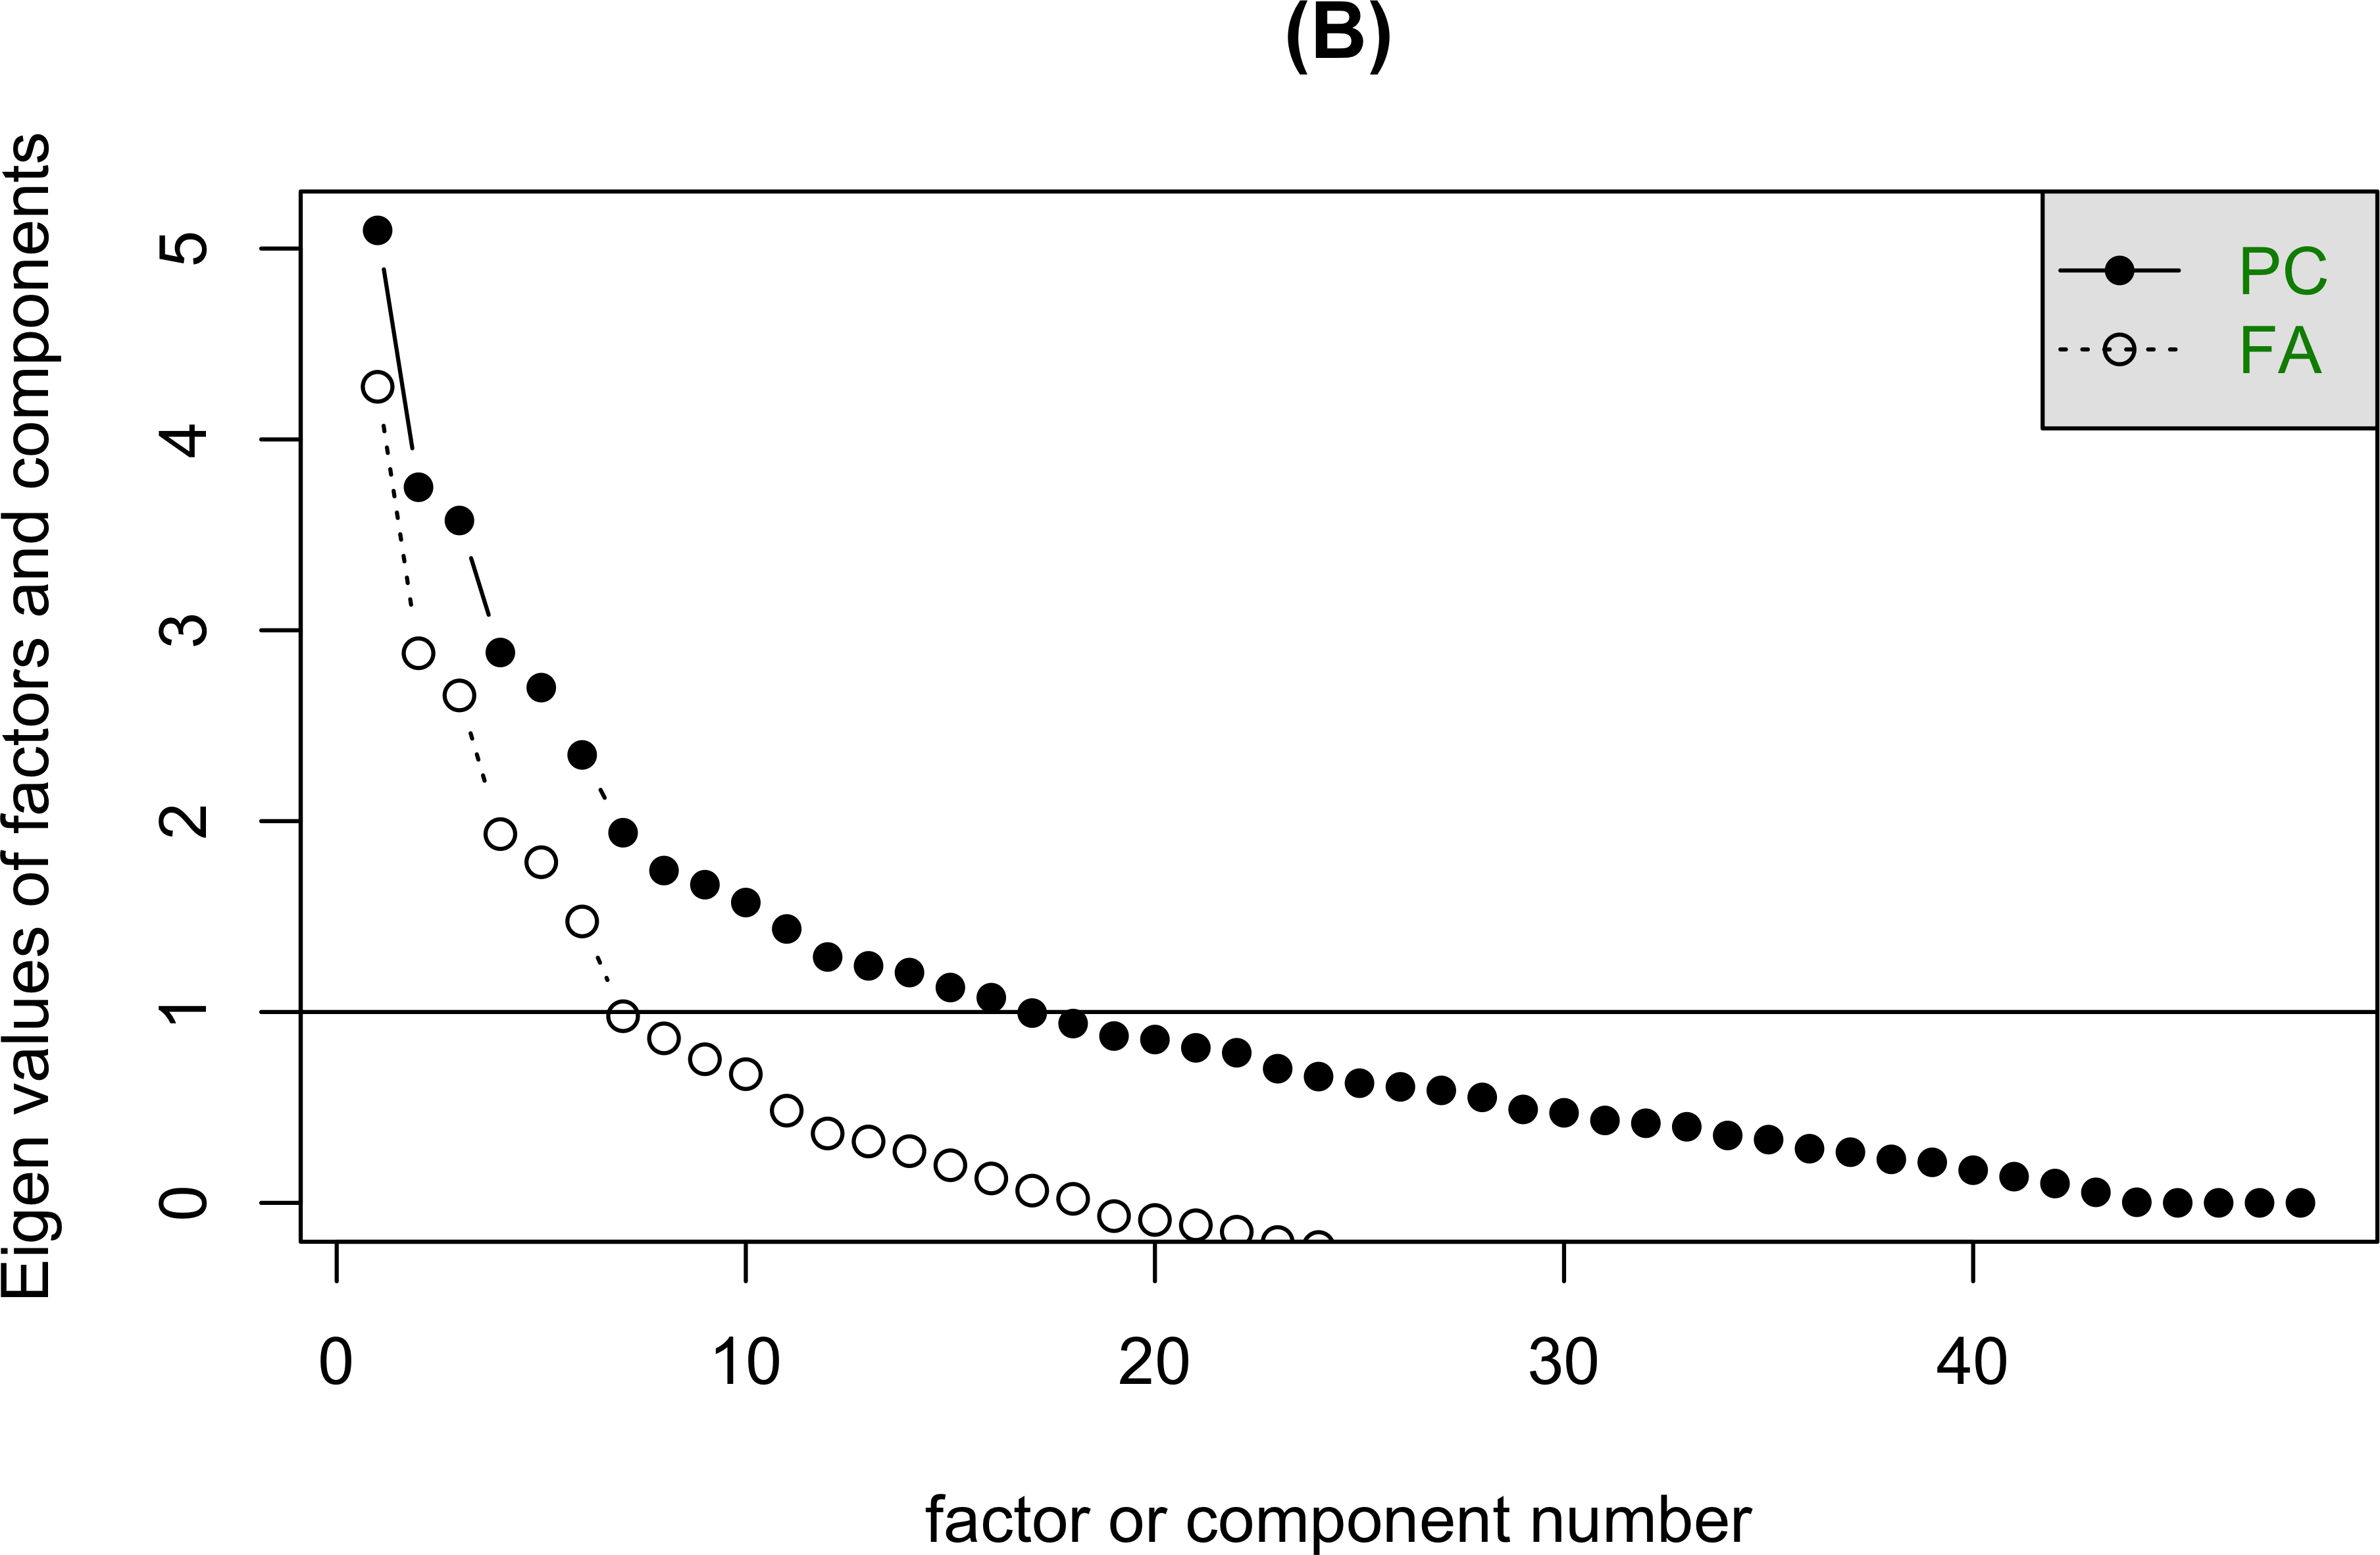
\includegraphics[width=0.5\linewidth,height=0.5\textheight]{manuscript_files/figure-latex/facid-2} 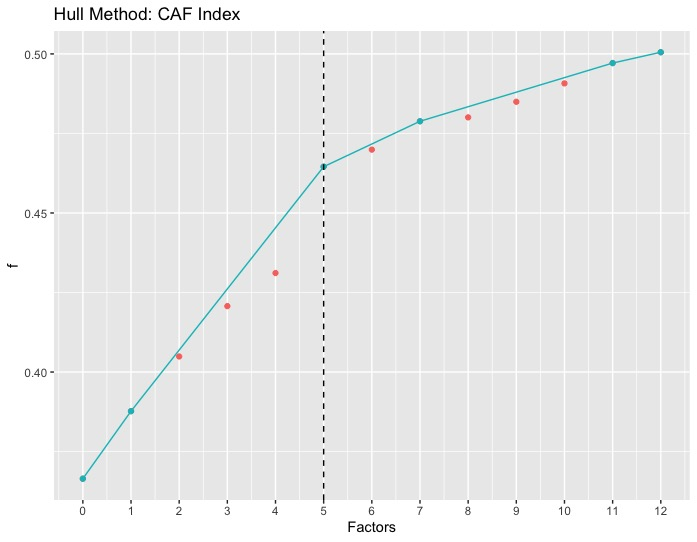
\includegraphics[width=0.5\linewidth,height=0.5\textheight]{HUll method} 

}

\caption{Factor Identification (A) Parallel analysis (B) Scree Plot, (C) Hull method}\label{fig:facid}
\end{figure}

\begin{figure}

{\centering 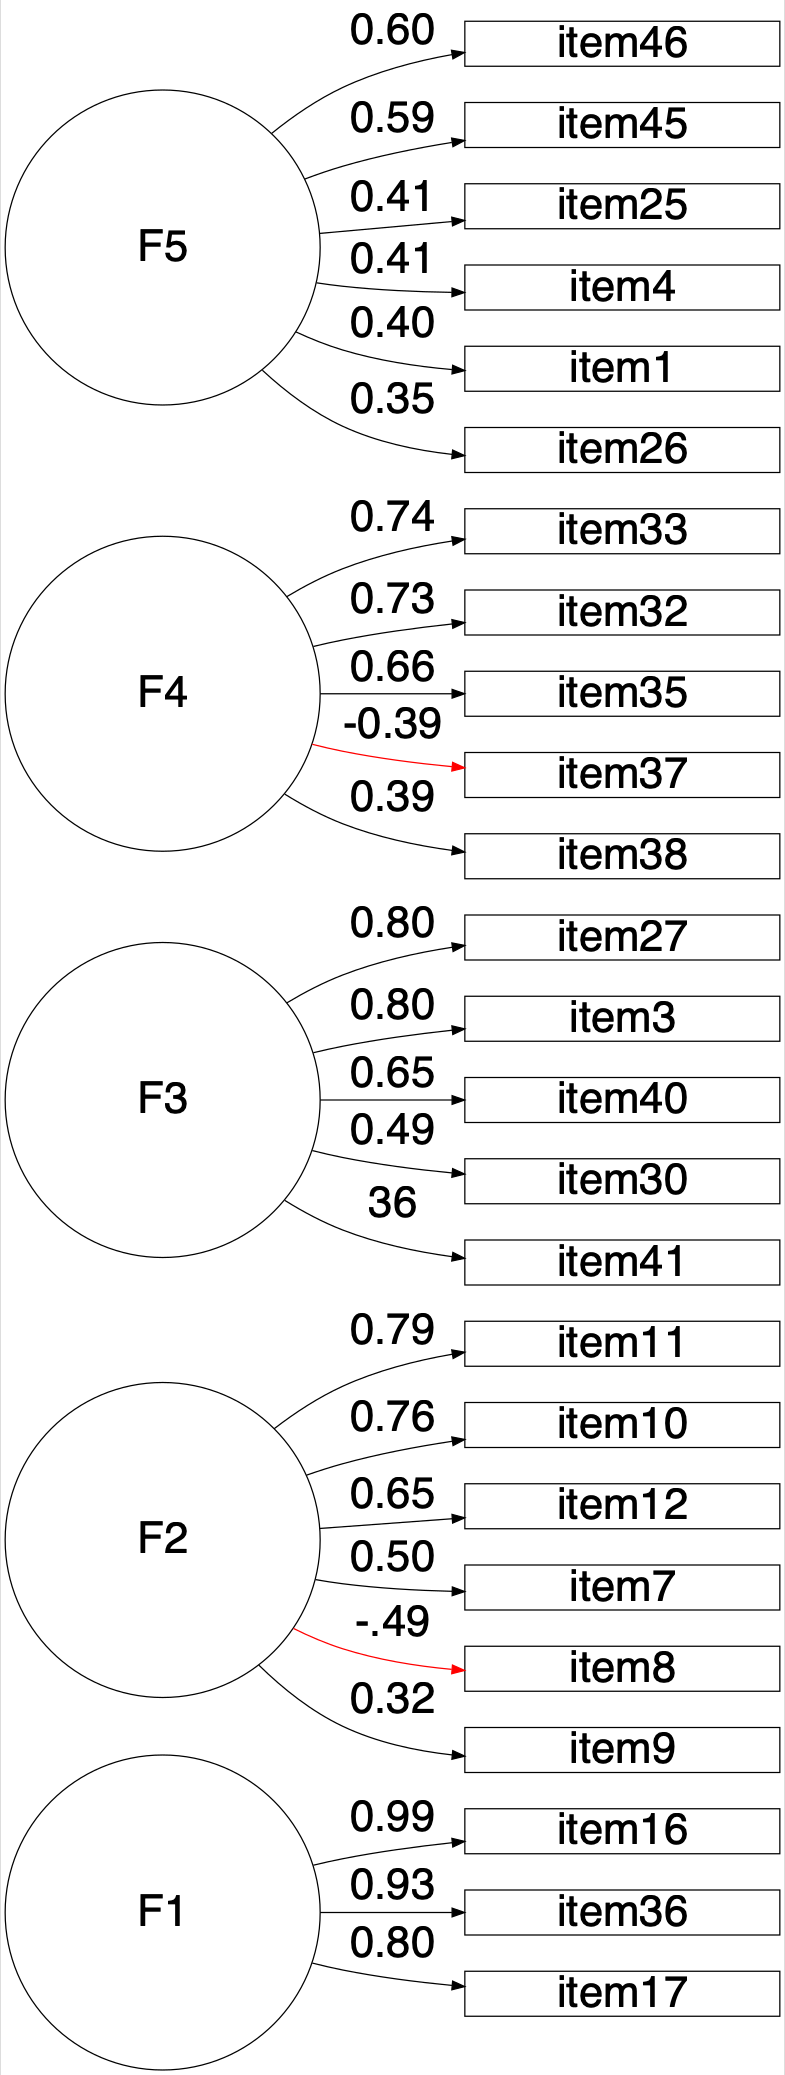
\includegraphics[width=1.2\linewidth,height=1\textheight]{EFAplot.LR} 

}

\caption{Five Factor Solution}\label{fig:EFAplot}
\end{figure}

The initial five-factor solution with all 48 items showed presence of cross-loading items (item 42, 16, \& 1) and poor factor loading (\textless.30) items (item 20, 3 ,15, 17, 40, 4, 11, 39, 18, 45, 29, 25, 8 , \& 46). At first, we discarded the items with poor factor-loading and ran another EFA on the remaining 34 items. This iteration of EFA also appeared as a misfit with items with poor factor-loading (Item 12, 22, 38, 6) and cross-loading (items 23, 31, 37, 48) . Another two rounds of EFA were conducted with gradually identifying problematic items and discarding them from the model. Finally, a five-factor EFA solution with 23 items was accepted with low RMSR = 0.04 (Brown, 2015), all factor-loading higher than .30 and no cross-loading greater than .30. We confirmed this five-factor latent structure using varimax rotation with a minimum residual extraction method (see the supplementary). Table\ref{tab:TabEFA5} displays the factor-loading (structural coefficients) and communality of the items. The absolute value of the factor-loading ranged from -.47 to .99 indicating strong coefficients. The commonalities ranged between .10 to .99. However, the histogram of the absolute values of non-redundant residual-correlations (Fig\ref{fig:Residuals} showed 26.09\% correlations greater than the absolute value of .05, indicating under-factoring. (C. D. Desjardins, 2018). Subsequently, we fitted a six-factor solution. However, a factor emerged with only two salient variable loading in the six-factor solution, thus disqualifying the six-factor solution.

In the five-factor solution, the first factor contained three items and explained 11\% of the total variance with a satisfactory internal reliability coefficient (\(\alpha\) =.86). All the items in this factor stemmed from the individual's preference to use blue light filters in different light environments. The second factor contained six items and explained 10\% of the total variance with a satisfactory internal reliability coefficient (\(\alpha\) =.71). Items under this factor commonly investigate an individual's hours spent outdoor. The third factor contained five items and explained 9\% of the total variance. Items under this factor dealt with the specific behaviors pertaining to sleep. However, the internal consistency reliability coefficient was not satisfactory (\(\alpha\) =.62). The fourth factor contained three items and explained 9\% of the total variance with a satisfactory internal consistency (\(\alpha\) =.77). These three items stemmed from the behavior related to an individual's cellphone usage during the sleep-wakeup time. Lastly, the fifth factor contained six items and explained 6\% of the total variance. Under this factor tried to measure an individual's behavior lead by the awareness of light's influence on health. However, this factor showed unsatisfactory internal consistency reliability (\(\alpha\) =.49). It is essential to attain a balance between psychometric properties and the interpretability of the common themes when exploring the latent structure. As all of the emerged factors are highly interpretable, regardless of the apparent low reliability of the two factors, we retain the five-factor solution with 23 items for our confirmatory factor analysis (CFA). Two items showed negative factor-loading (items 44 and 21). Upon inspection, it was understood that these items are negatively correlated to the common theme, and thus in the CFA analysis, we reversed the response code for these two items.

\begin{table}[tbp]

\begin{center}
\begin{threeparttable}

\caption{\label{tab:TabEFA5}}

\begin{tabular}{ccccccc}
\toprule
 & \multicolumn{1}{c}{F1} & \multicolumn{1}{c}{F2} & \multicolumn{1}{c}{F3} & \multicolumn{1}{c}{F4} & \multicolumn{1}{c}{F5} & \multicolumn{1}{c}{Communality}\\
\midrule
item43 & 0.99 & - & - & - & - & 0.99\\
item26 & 0.93 & - & - & - & - & 0.9\\
item32 & 0.8 & - & - & - & - & 0.67\\
item10 & - & 0.82 & - & - & - & 0.68\\
item47 & - & 0.82 & - & - & - & 0.7\\
item36 & - & 0.63 & - & - & - & 0.45\\
item44 & - & -0.47 & - & - & - & 0.24\\
item35 & - & 0.46 & - & - & - & 0.24\\
item13 & - & 0.34 & - & - & - & 0.13\\
item14 & - & - & 0.89 & - & - & 0.81\\
item41 & - & - & 0.7 & - & - & 0.6\\
item7 & - & - & 0.66 & - & - & 0.45\\
item27 & - & - & 0.38 & - & - & 0.21\\
item21 & - & - & -0.34 & - & - & 0.12\\
item34 & - & - & - & 0.84 & - & 0.74\\
item19 & - & - & - & 0.8 & - & 0.64\\
item2 & - & - & - & 0.67 & - & 0.54\\
item5 & - & - & - & - & 0.69 & 0.51\\
item24 & - & - & - & - & 0.54 & 0.33\\
item30 & - & - & - & - & 0.52 & 0.29\\
item1 & - & - & - & - & 0.35 & 0.13\\
item16 & - & - & - & - & 0.31 & 0.21\\
item28 & - & - & - & - & 0.31 & 0.1\\
\% of variance & 11 & 10 & 9 & 9 & 6 & -\\
\bottomrule
\addlinespace
\end{tabular}

\begin{tablenotes}[para]
\normalsize{\textit{Note.} Only loading higher than .30 is reported}
\end{tablenotes}

\end{threeparttable}
\end{center}

\end{table}

\begin{figure}

{\centering 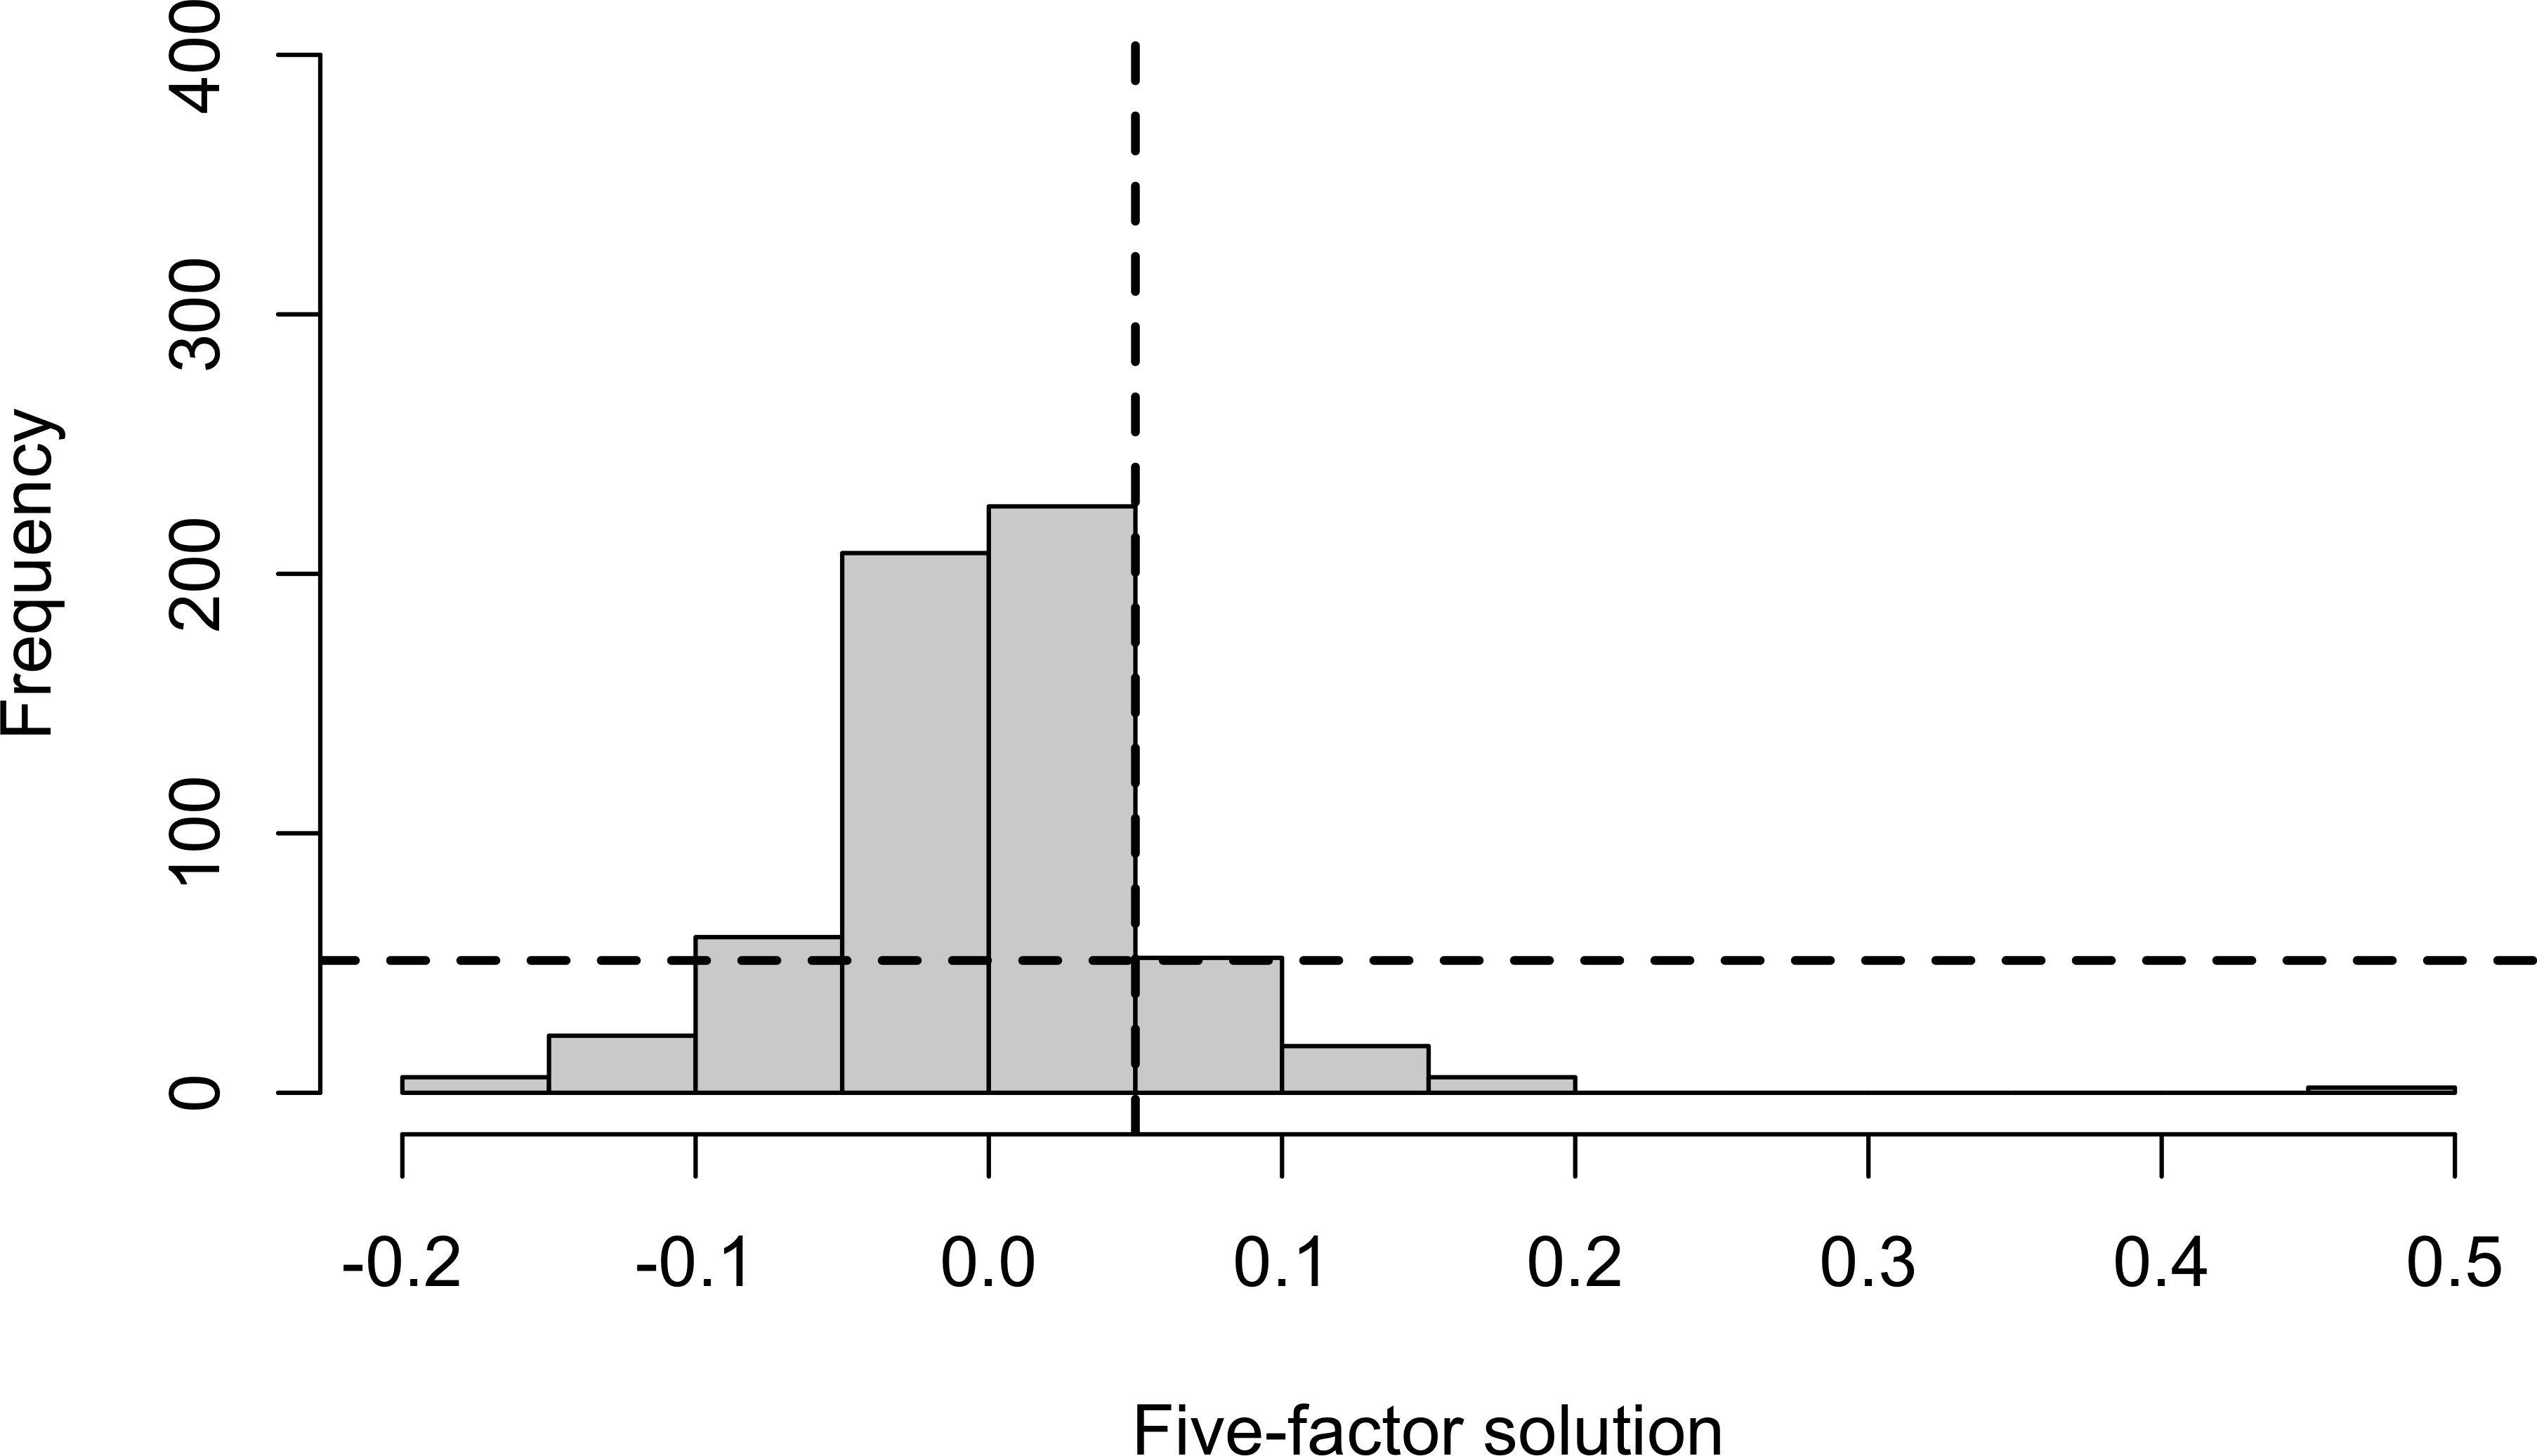
\includegraphics[width=0.5\linewidth,height=0.5\textheight]{manuscript_files/figure-latex/Residuals-1} 

}

\caption{ Histogram of residulas:  five-factor solution}\label{fig:Residuals}
\end{figure}

\hypertarget{confirmatory-factor-analysis}{%
\section{Confirmatory Factor Analysis}\label{confirmatory-factor-analysis}}

\hypertarget{irt}{%
\subsection{IRT}\label{irt}}

\hypertarget{discussion}{%
\section{Discussion}\label{discussion}}

\newpage

\hypertarget{references}{%
\section{References}\label{references}}

\begingroup
\setlength{\parindent}{-0.5in}
\setlength{\leftskip}{0.5in}

\hypertarget{refs}{}
\begin{CSLReferences}{1}{0}
\leavevmode\hypertarget{ref-R-papaja}{}%
Aust, F., \& Barth, M. (2020). \emph{{papaja}: {Prepare} reproducible {APA} journal articles with {R Markdown}}. Retrieved from \url{https://github.com/crsh/papaja}

\leavevmode\hypertarget{ref-bakerBasicsItemResponse2017}{}%
Baker, F. B. (2017). \emph{The {Basics} of {Item Response Theory Using R}} (1st ed. 2017.). {Springer}.

\leavevmode\hypertarget{ref-bandalosFactorAnalysisExploratory2018}{}%
Bandalos, D. L., \& Finney, S. J. (2018). Factor analysis: {Exploratory} and confirmatory. In \emph{The reviewer's guide to quantitative methods in the social sciences} (pp. 98--122). {Routledge}.

\leavevmode\hypertarget{ref-R-tinylabels}{}%
Barth, M. (2021). \emph{{tinylabels}: Lightweight variable labels}. Retrieved from \url{https://github.com/mariusbarth/tinylabels}

\leavevmode\hypertarget{ref-bartlettNoteMultiplyingFactors1954}{}%
Bartlett, M. (1954). A {Note} on the {Multiplying Factors} for {Various Chi}-square {Approximations}. \emph{Journal of the Royal Statistical Society. Series B, Methodological}, \emph{16}(2), 296--298.

\leavevmode\hypertarget{ref-bentlerPracticalIssuesStructural1987}{}%
Bentler, P. M., \& Chou, C.-P. (1987). Practical {Issues} in {Structural Modeling}. \emph{Sociological Methods \& Research}, \emph{16}(1), 78--117. \url{https://doi.org/10.1177/0049124187016001004}

\leavevmode\hypertarget{ref-brownConfirmatoryFactorAnalysis2015}{}%
Brown, T. A. (2015). \emph{Confirmatory factor analysis for applied research} (2nd ed.). {New York, NY, US}: {The Guilford Press}.

\leavevmode\hypertarget{ref-R-MOTE}{}%
Buchanan, E. M., Gillenwaters, A., Scofield, J. E., \& Valentine, K. D. (2019). \emph{{MOTE: Measure of the Effect}: Package to assist in effect size calculations and their confidence intervals}. Retrieved from \url{http://github.com/doomlab/MOTE}

\leavevmode\hypertarget{ref-cattellScreeTestNumber1966}{}%
Cattell, R. B. (1966). The {Scree Test For The Number Of Factors}. \emph{Multivariate Behavioral Research}, \emph{1}(2), 245--276. \url{https://doi.org/10.1207/s15327906mbr0102_10}

\leavevmode\hypertarget{ref-R-shiny}{}%
Chang, W., Cheng, J., Allaire, J., Sievert, C., Schloerke, B., Xie, Y., \ldots{} Borges, B. (2021). \emph{Shiny: Web application framework for r}. Retrieved from \url{https://CRAN.R-project.org/package=shiny}

\leavevmode\hypertarget{ref-comreyFirstCourseFactor1992}{}%
Comrey, A. L., \& Lee, H. B. (1992). \emph{A first course in factor analysis, 2nd ed}. {Hillsdale, NJ, US}: {Lawrence Erlbaum Associates, Inc}.

\leavevmode\hypertarget{ref-desjardinsHandbookEducationalMeasurement2018}{}%
Desjardins, C., \& Bulut, O. (2018). \emph{Handbook of {Educational Measurement} and {Psychometrics Using R}}. \url{https://doi.org/10.1201/b20498}

\leavevmode\hypertarget{ref-desjardinsHandbookEducationalMeasurement2018a}{}%
Desjardins, C. D. (2018). \emph{Handbook of educational measurement and psychometrics using {R}} (O. Bulut \& ProQuest (Firm), Eds.). {Boca Raton, FL : CRC Press}.

\leavevmode\hypertarget{ref-R-paran}{}%
Dinno, A. (2018). \emph{Paran: Horn's test of principal components/factors}. Retrieved from \url{https://CRAN.R-project.org/package=paran}

\leavevmode\hypertarget{ref-R-semPlot}{}%
Epskamp, S. (2019). \emph{semPlot: Path diagrams and visual analysis of various SEM packages' output}. Retrieved from \url{https://CRAN.R-project.org/package=semPlot}

\leavevmode\hypertarget{ref-R-qgraph}{}%
Epskamp, S., Cramer, A. O. J., Waldorp, L. J., Schmittmann, V. D., \& Borsboom, D. (2012). {qgraph}: Network visualizations of relationships in psychometric data. \emph{Journal of Statistical Software}, \emph{48}(4), 1--18.

\leavevmode\hypertarget{ref-R-purrr}{}%
Henry, L., \& Wickham, H. (2020). \emph{Purrr: Functional programming tools}. Retrieved from \url{https://CRAN.R-project.org/package=purrr}

\leavevmode\hypertarget{ref-hornRationaleTestNumber1965}{}%
Horn, J. L. (1965). A rationale and test for the number of factors in factor analysis. \emph{Psychometrika}, \emph{30}(2), 179--185. \url{https://doi.org/10.1007/BF02289447}

\leavevmode\hypertarget{ref-hutchesonMultivariateSocialScientist1999}{}%
Hutcheson, G. D. (1999). \emph{The multivariate social scientist : Introductory statistics using generalized linear models}. {London : SAGE}.

\leavevmode\hypertarget{ref-R-DiagrammeRsvg}{}%
Iannone, R. (2016). \emph{DiagrammeRsvg: Export DiagrammeR graphviz graphs as SVG}. Retrieved from \url{https://CRAN.R-project.org/package=DiagrammeRsvg}

\leavevmode\hypertarget{ref-R-DiagrammeR}{}%
Iannone, R. (2021). \emph{DiagrammeR: Graph/network visualization}. Retrieved from \url{https://github.com/rich-iannone/DiagrammeR}

\leavevmode\hypertarget{ref-jacksonRevisitingSampleSize2003}{}%
Jackson, D. L. (2003). Revisiting {Sample Size} and {Number} of {Parameter Estimates}: {Some Support} for the {N}:q {Hypothesis}. \emph{Structural Equation Modeling}, \emph{10}(1), 128--141. \url{https://doi.org/10.1207/S15328007SEM1001_6}

\leavevmode\hypertarget{ref-R-semTools}{}%
Jorgensen, T. D., Pornprasertmanit, S., Schoemann, A. M., \& Rosseel, Y. (2021). \emph{\texttt{semTools}: {U}seful tools for structural equation modeling}. Retrieved from \url{https://CRAN.R-project.org/package=semTools}

\leavevmode\hypertarget{ref-kaiserIndexFactorialSimplicity1974}{}%
Kaiser, H. F. (1974). An index of factorial simplicity. \emph{Psychometrika}, \emph{39}(1), 31--36. \url{https://doi.org/10.1007/bf02291575}

\leavevmode\hypertarget{ref-R-ggcorrplot}{}%
Kassambara, A. (2019). \emph{Ggcorrplot: Visualization of a correlation matrix using 'ggplot2'}. Retrieved from \url{https://CRAN.R-project.org/package=ggcorrplot}

\leavevmode\hypertarget{ref-klinePrinciplesPracticeStructural2015}{}%
Kline, R. B. (2015). \emph{Principles and practice of structural equation modeling}. {The Guilford Press}.

\leavevmode\hypertarget{ref-lorenzo-sevaHullMethodSelecting2011}{}%
Lorenzo-Seva, U., Timmerman, M., \& Kiers, H. (2011). The {Hull Method} for {Selecting} the {Number} of {Common Factors}. \emph{Multivariate Behavioral Research}, \emph{46}, 340--364. \url{https://doi.org/10.1080/00273171.2011.564527}

\leavevmode\hypertarget{ref-R-correlation}{}%
Makowski, D., Ben-Shachar, M. S., Patil, I., \& Lüdecke, D. (2020). Methods and algorithms for correlation analysis in r. \emph{Journal of Open Source Software}, \emph{5}(51), 2306. \url{https://doi.org/10.21105/joss.02306}

\leavevmode\hypertarget{ref-mardiaMeasuresMultivariateSkewness1970}{}%
Mardia, K. V. (1970). Measures of multivariate skewness and kurtosis with applications. \emph{Biometrika}, \emph{57}(3), 519--530. \url{https://doi.org/10.1093/biomet/57.3.519}

\leavevmode\hypertarget{ref-R-tibble}{}%
Müller, K., \& Wickham, H. (2021). \emph{Tibble: Simple data frames}. Retrieved from \url{https://CRAN.R-project.org/package=tibble}

\leavevmode\hypertarget{ref-R-EFA.MRFA}{}%
Navarro-Gonzalez, D., \& Lorenzo-Seva, U. (2021). \emph{EFA.MRFA: Dimensionality assessment using minimum rank factor analysis}. Retrieved from \url{https://CRAN.R-project.org/package=EFA.MRFA}

\leavevmode\hypertarget{ref-R-rsvg}{}%
Ooms, J. (2021). \emph{Rsvg: Render SVG images into PDF, PNG, PostScript, or bitmap arrays}. Retrieved from \url{https://CRAN.R-project.org/package=rsvg}

\leavevmode\hypertarget{ref-R-base}{}%
R Core Team. (2021). \emph{R: A language and environment for statistical computing}. Vienna, Austria: R Foundation for Statistical Computing. Retrieved from \url{https://www.R-project.org/}

\leavevmode\hypertarget{ref-R-psych}{}%
Revelle, W. (2021). \emph{Psych: Procedures for psychological, psychometric, and personality research}. Evanston, Illinois: Northwestern University. Retrieved from \url{https://CRAN.R-project.org/package=psych}

\leavevmode\hypertarget{ref-R-lavaan}{}%
Rosseel, Y. (2012). {lavaan}: An {R} package for structural equation modeling. \emph{Journal of Statistical Software}, \emph{48}(2), 1--36. Retrieved from \url{https://www.jstatsoft.org/v48/i02/}

\leavevmode\hypertarget{ref-R-dlookr}{}%
Ryu, C. (2021). \emph{Dlookr: Tools for data diagnosis, exploration, transformation}. Retrieved from \url{https://CRAN.R-project.org/package=dlookr}

\leavevmode\hypertarget{ref-schonbrodtWhatSampleSize2013}{}%
Schönbrodt, F. D., \& Perugini, M. (2013). At what sample size do correlations stabilize? \emph{Journal of Research in Personality}, \emph{47}(5), 609--612. \url{https://doi.org/10.1016/j.jrp.2013.05.009}

\leavevmode\hypertarget{ref-shapiroAnalysisVarianceTest1965}{}%
Shapiro, S. S., \& Wilk, M. B. (1965). An analysis of variance test for normality (complete samples). \emph{Biometrika}, \emph{52}(3-4), 591--611. \url{https://doi.org/10.1093/biomet/52.3-4.591}

\leavevmode\hypertarget{ref-velicerDeterminingNumberComponents1976}{}%
Velicer, W. (1976). Determining the {Number} of {Components} from the {Matrix} of {Partial Correlations}. \emph{Psychometrika}, \emph{41}, 321--327. \url{https://doi.org/10.1007/BF02293557}

\leavevmode\hypertarget{ref-R-MASS}{}%
Venables, W. N., \& Ripley, B. D. (2002). \emph{Modern applied statistics with s} (Fourth). New York: Springer. Retrieved from \url{https://www.stats.ox.ac.uk/pub/MASS4/}

\leavevmode\hypertarget{ref-watkinsStepbyStepGuideExploratory2020}{}%
Watkins, M. (2020). \emph{A {Step}-by-{Step Guide} to {Exploratory Factor Analysis} with {R} and {RStudio}}. \url{https://doi.org/10.4324/9781003120001}

\leavevmode\hypertarget{ref-R-ggplot2}{}%
Wickham, H. (2016). \emph{ggplot2: Elegant graphics for data analysis}. Springer-Verlag New York. Retrieved from \url{https://ggplot2.tidyverse.org}

\leavevmode\hypertarget{ref-R-stringr}{}%
Wickham, H. (2019). \emph{Stringr: Simple, consistent wrappers for common string operations}. Retrieved from \url{https://CRAN.R-project.org/package=stringr}

\leavevmode\hypertarget{ref-R-forcats}{}%
Wickham, H. (2021a). \emph{Forcats: Tools for working with categorical variables (factors)}. Retrieved from \url{https://CRAN.R-project.org/package=forcats}

\leavevmode\hypertarget{ref-R-tidyr}{}%
Wickham, H. (2021b). \emph{Tidyr: Tidy messy data}. Retrieved from \url{https://CRAN.R-project.org/package=tidyr}

\leavevmode\hypertarget{ref-R-tidyverse}{}%
Wickham, H., Averick, M., Bryan, J., Chang, W., McGowan, L. D., François, R., \ldots{} Yutani, H. (2019). Welcome to the {tidyverse}. \emph{Journal of Open Source Software}, \emph{4}(43), 1686. \url{https://doi.org/10.21105/joss.01686}

\leavevmode\hypertarget{ref-R-readxl}{}%
Wickham, H., \& Bryan, J. (2019). \emph{Readxl: Read excel files}. Retrieved from \url{https://CRAN.R-project.org/package=readxl}

\leavevmode\hypertarget{ref-R-dplyr}{}%
Wickham, H., François, R., Henry, L., \& Müller, K. (2021). \emph{Dplyr: A grammar of data manipulation}. Retrieved from \url{https://CRAN.R-project.org/package=dplyr}

\leavevmode\hypertarget{ref-R-readr}{}%
Wickham, H., \& Hester, J. (2021). \emph{Readr: Read rectangular text data}. Retrieved from \url{https://CRAN.R-project.org/package=readr}

\leavevmode\hypertarget{ref-worthingtonScaleDevelopmentResearch2006}{}%
Worthington, R. L., \& Whittaker, T. A. (2006). Scale {Development Research}: {A Content Analysis} and {Recommendations} for {Best Practices}. \emph{The Counseling Psychologist}, \emph{34}(6), 806--838. \url{https://doi.org/10.1177/0011000006288127}

\leavevmode\hypertarget{ref-R-kableExtra}{}%
Zhu, H. (2021). \emph{kableExtra: Construct complex table with 'kable' and pipe syntax}. Retrieved from \url{https://CRAN.R-project.org/package=kableExtra}

\end{CSLReferences}

\endgroup


\end{document}
